% roboto, callout, [[speech bubble]], sans, [[append after command]], sfdefault, arc, [[block diagram]]
\documentclass[tikz,border=2]{standalone}
\usetikzlibrary{shadows,arrows,shapes,positioning,calc,backgrounds,fit,automata}
%
%%%%%%%%%%%%%%%%%%%%%%%%%%%%%%%%%%%%
%% Common preamble
%%%%%%%%%%%%%%%%%%%%%%%%%%%%%%%%%%%%
% PAGE
%% \usepackage{fullpage}
% FONTS
%%\usepackage{lmodern} % enhanced version of computer modern
\usepackage[sfdefault]{noto}
\usepackage[T1]{fontenc} % for hyphenated characters
%% \usepackage{gillius2}
%% \renewcommand{\familydefault}{\sfdefault}
\usepackage{amssymb} % for \checkmark
\usepackage{mathtools} % contains amsmath which comes with align
\usepackage{amsthm}
%%\usepackage{enumitem}
\usepackage{microtype} % some compression
%%%%%%%%%%%%%%%%%%%%%%%%%%%%%%%%%%%%
\usepackage{subfig}
\usepackage{tikz}
\usetikzlibrary{spy,shadows,arrows,shapes,positioning,calc,backgrounds,fit,automata}
\newcommand{\score}{\text{score}}

\definecolor{Green}{HTML}{BCD695}
\definecolor{Darkgreen}{HTML}{0092A0}
\definecolor{Darkbrown}{HTML}{474342}
\definecolor{Brown}{HTML}{6C6B67}
\definecolor{Lightbrown}{HTML}{A3A5A6}
\definecolor{Lighterbrown}{HTML}{E0DCDB}


\newcommand{\dunder}[1]{\underline{\underline{#1}}}
\newcommand{\dmax}{d_{\max}}
\newcommand{\cost}{\text{cost}}
%\newcommand{\comment}[1]{{\color{red}#1}}
\newcommand{\wmin}{w_{\min}}
\newcommand{\copt}{C_{\text{OPT}}}
\newcommand{\TikZ}{Ti\textit{k}Z\xspace}
\newcommand{\tuta}{\emph{T. absoluta}}
\newcommand{\prempt}{\textsc{PREMpT}}
\newcommand{\parnode}[1]{\parbox{3cm}{\centering #1}}

%%
%% This ``scales'' the font. Don't extend too much beyond 128x96
%% Uncomment the next line for default sizes:
%% \setbeamercolor{block title}{use=structure,fg=white,bg=black!75!white}
%% \setbeamercolor{block body}{use=structure,fg=black,bg=black!10!white}
%%
%% ----------------------------------------------------------------------
%%
\begin{document}
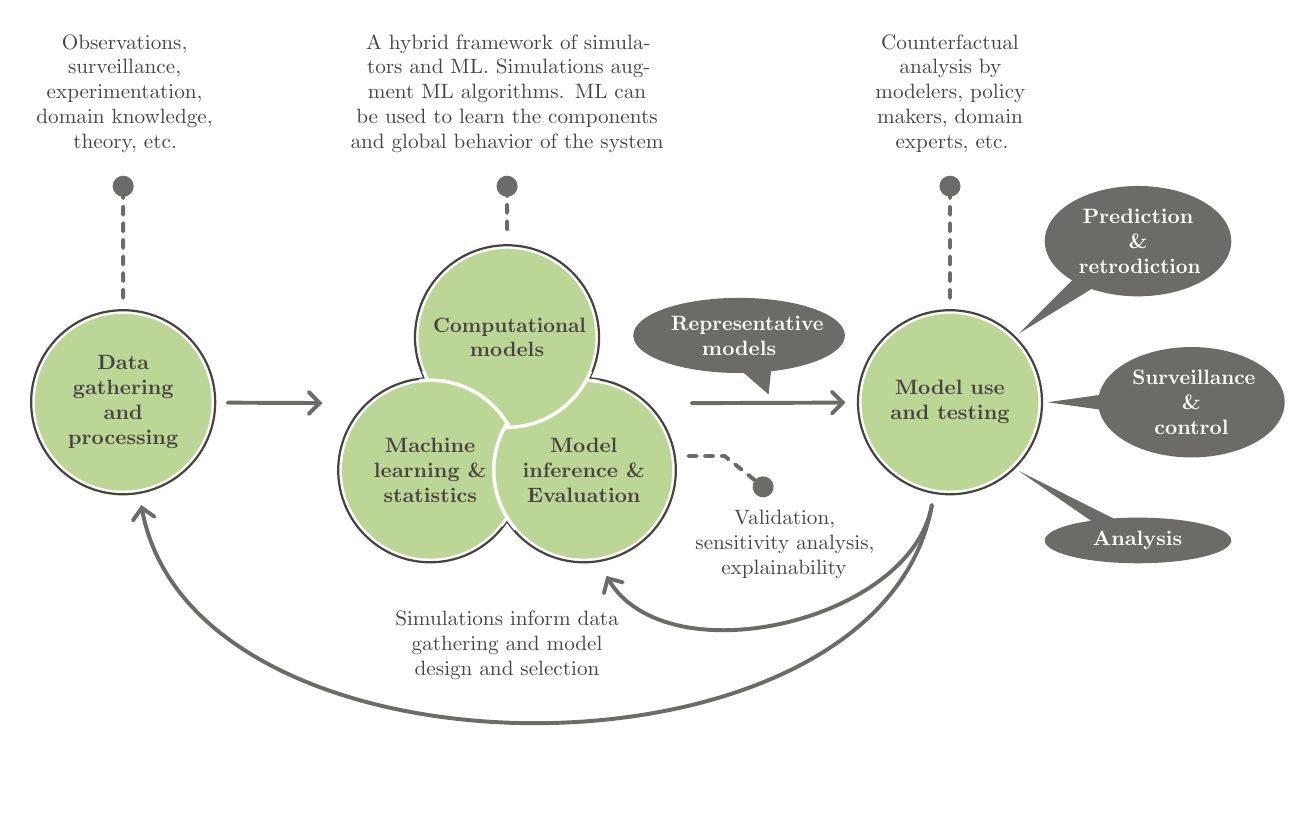
\begin{tikzpicture}
[scale=.75,auto,transform shape,
    edge/.style={line cap=round,Brown,>=angle 90, shorten >=2mm, shorten <=2mm, line
    width=.5mm},
every node/.style={text=Darkbrown},
explain/.style={align=center,text width=3cm,text=Darkbrown},
callout/.style={align=center,font=\bfseries,text
width=2cm,fill=Brown,text=white,ellipse callout},
block/.style={font=\bfseries,text width=2.5cm,circle,align=center,minimum width=3cm,inner sep=0mm,draw=white,ultra thin,fill=Green, append after
command={\pgfextra{\node[draw=Darkbrown,fill=none,circle,inner sep=-3mm,thick,fit=(\tikzlastnode)]{};}}},
dedge/.style={line cap=round,line width=.5mm,shorten >=2mm, shorten
<=2mm,Brown,dashed}]

\node[block] (data) {Data \\gathering \\and \\processing};

\begin{scope}[shift={(6.5,1.1)},local bounding box=AI]
\node[block] at (0,0) {Computational \\ models};
% sqrt(3)*radius
\node[block] at (240:2.6) {Machine learning \& statistics};
\node[block] at (-60:2.6) {Model \\ inference \& Evaluation};
%% remove dark green lines
\draw[Green,line width=2.5mm] ([shift=(87:1.5)]-60:2.6) arc (87:213:1.5);
\draw[Green,line width=2.5mm] ([shift=(93.5:1.5)]240:2.6) arc (93.5:30:1.5);
%% add white lines
\draw[white,line width=.45mm] ([shift=(-92:1.525)]0,0) arc (-92:-22:1.525);
\draw[white,line width=.45mm] ([shift=(97:1.525)]240:2.6) arc (97:28.5:1.525);
\draw[white,line width=.45mm] ([shift=(149:1.525)]-60:2.6) arc (149:221:1.525);
%% remove irritating light green lines
\draw[white,line width=.4mm] ([shift=(208:1.525)]0:0) arc (208:202:1.525);
\draw[white,line width=.4mm] ([shift=(-32:1.525)]240:2.6) arc (-32:-38:1.525);
\draw[white,line width=.4mm,white] ([shift=(89:1.525)]-60:2.6) arc (89:80:1.525);
\node[circle,inner sep=.5,fill=white] at (0,-1.5) {};
\end{scope}

\node[block] (sim) at (14,0) {Model use and testing};

\draw (data) edge[edge,->] (AI);
\draw[->] (AI) edge[edge] node (dummy) {} (sim); 
\node [callout,above of=dummy,callout absolute
pointer=(dummy),text width=2.3cm,shift={(-.5,0)}] {Representative models};
\draw (sim) edge[edge,->,out=260,in=-80] (data);
\draw (sim) edge[edge,->,out=260,in=-60] (AI);
%% 
%% explanation starts here
%%
%%\node[explain,below=of AI,shift={(0,.9)}] (abd) {\Large \bf Abductive loop}; 
\node[explain,below=of AI,shift={(0,.3)},text width=4cm] (abd) {Simulations
inform data gathering and model design and selection};

\node[explain,anchor=south,above=of data,shift={(0,1.6)}] (edata) {Observations,
surveillance, experimentation, domain knowledge, theory, etc.};
\draw[dedge,-*] (data) -- (edata);
%%
\node[explain,anchor=south,text width=6cm] (eAI) at
(AI|-edata.south) {A hybrid framework of simulators and ML.
Simulations augment ML algorithms. ML can be used to learn the components
and global behavior of the system};
\draw[dedge,-*] (AI) -- (eAI);
%%
\node[explain,below right=of AI,shift={(-.8,2)}] (eeval) {Validation,
sensitivity analysis, explainability};
\draw[dedge,*-] (eeval.north) -- ++(-1,.8) -- +(-1,0);
%%
\node[explain,anchor=south] (esim) at (sim|-edata.south) {
Counterfactual analysis by modelers, policy makers, domain experts, etc.};
\draw[dedge,-*] (sim) -- (esim);
%%

%% outcomes
\node (a1) at ([shift={(.1,.1)}]sim.north east) {};
\node (a2) at ([shift={(.15,0)}]sim.east) {};
\node (a3) at ([shift={(.1,-.1)}]sim.south east) {};
\node[callout,above right=of sim,callout absolute pointer=(a1)] (pred)
{Prediction \\\&\\ retrodiction};
\node[callout,right=of sim,callout absolute pointer=(a2)] (dec)
{Surveillance \\\&\\ control};
\node[callout,below right=of sim,callout absolute pointer=(a3)]
(so) {Analysis};

\end{tikzpicture}
\end{document}

